\section{Densidad, Presión y Temperatura}
\subsection*{Densidad}
\subsubsection*{Densidad Absoluta}
La densidad es una magnitud referida a la cantidad de masa contenida en un determinado volumen, y puede utilizarse en términos absolutos o relativos.
\begin{Theorem*} {Definición - Densidad absoluta}
	La densidad absoluta o densidad normal o simplemente densidad, expresa la masa por unidad de volumen.
	$$ \rho=\frac{m}{V} $$
\end{Theorem*}
\subsubsection*{Densidad de una mezcla}
Para una mezcla homogénea o heterogénea su masa y volumen se establecen como la suma de sus componentes:
$$ m_M = \sum_{i=1}^{n}mi=m_1+m_2+m_3+\cdots+m_n $$
$$ V_M = \sum_{i=1}^{n}Vi=V_1+V_2+V_3+\cdots+V_n $$
Sin embargo su densidad se deberá establecer como la relación entre la masa total y el volumen:
\begin{Theorem*} {Densidad de una mezcla}
	Sea una mezcla homogénea o heterogénea, su densidad se establece como la suma entre la relación entre ls masa y volumen de cada componente.
	$$\rho_M=\sum_{i=1}^{n}\frac{m_i}{V_i}$$
	Es decir:
	$$\rho_M=\frac{m_{total}}{V_{total}}=\frac{m_1+m_2+m_3+\cdots+m_n}{V_1+V_2+V_3+\cdots+V_n}$$
\end{Theorem*}
Asi tambien, tener en cuenta que cada componente mantiene intacta sus propiedades fisicas, por lo tanto tendremos para la sustancia i:
$$ \rho_i = \frac{m_i}{V_i} \Rightarrow m_i=\rho_iV_i $$
Analogamente podemos estables la densidad de la mezcla de la siguiente manera:
$$ \rho_M = \sum_{i=1}^{n} \frac{\rho_iV_i}{V_i}=\frac{\rho_1V_1+\rho_2V_2+\cdots+\rho_nV_n}{V_1+V_2+\cdots+V_n} $$
\subsubsection*{Peso especifico}
\begin{Theorem*} {Peso especifico}
	Es un propiedad intensiva, que mide el peso de una sustancia por unidad de volumen:
	$$ \gamma=\frac{W}{V} $$
	donde $V$ es volumen y $W$ es peso.
\end{Theorem*}
Las unidades el peso especifico en SI son: $\mathrm{\left[\frac{N}{m^3}\right]}$ o $\mathrm{\left[\frac{Newton}{metro cubico}\right]}$ y en CGS son: $\mathrm{\left[\frac{g_f}{cc}\right]}$ o $\mathrm{\left[\frac{gramo-fuerza}{centimetro cubico}\right]}$.
Un punto muy importante es que el peso especifico es numericamente igual a la densidad.
\begin{Theorem*} {El peso especifico y densidad}
	El peso especifico expresado en unidades técnicas es numéricamente igual a la densidad expresada en unidades absolutas:
	$$ \rho = \gamma \quad \text{(numéricamente)} $$
	siempre que la gravedad sea constante.
\end{Theorem*}
\subsubsection*{Densidad relativa}
\begin{Theorem*} {Densidad relativa}
	También llamada gravedad especifica, es la relación entre la densidad de una sustancia y la densidad de otra tomada como referencia denominada sustancia patrón.
	$$ \rho_r=\frac{\rho}{\rho_{ref}} $$
\end{Theorem*}
cabe resaltar puntos importante con respecto a la densidad relativa
\begin{itemize}
	\item $\rho_r$ es adimensional.
	\item La sustancia patrón para líquidos y sólidos es el agua ($\rho_{\ch{H2O}}=1\mathrm{[g/cc]}$ en condiciones normales).
	\item La sustancia patron para gases o vapores es el aire ($\rho_{aire}=1.29\mathrm{[g/L]}$ en condiciones normales).
\end{itemize}
Otro punto igual de importante pero sobre todo útil que la igualdad numérica con el peso especifico e implícitamente con la densidad.
\begin{Theorem*} {La densidad relativa y el peso especifico}
	Para sustancias solidas y liquidas, considerando también el enunciado de \textit{El peso especifico y densidad}. La densidad relativa es numéricamente igual al peso especifico e implícitamente a la densidad.
	$$ \rho=\gamma=\rho_r \quad \text{(numéricamente)} $$
\end{Theorem*}
\subsection*{Presión}
\begin{Theorem*} {Definición - Presión}
	Es la medida del efecto de la distribución de fuerzas normales (perpendiculares) aplicada sobre una superficie o área
	$$ P = \frac{N}{A} $$
	donde $N$ son fuerzas normales con respecto a la área $A$.
\end{Theorem*}
\subsubsection*{Presión hidrostática}
\begin{Theorem*} {Presión hidrostática}
	Es la presión que ejerce un liquido en reposo, sobre un punto y se define de la siguiente manera:
	$$ P_L=\gamma_L\cdot y=\rho_L\cdot g\cdot y $$
	donde $y$ representa la profundidad donde se mide (altura).
\end{Theorem*}
\subsubsection*{Presion atmosferica}
Es la presion que ejerce la atmosfera sobre la superficie terrestre en un punto determinado.
Donde su valor depende ciertas condiciones, sin embargo su valor en condiciones normales es:
$$ P_{atm}^{CN}=760\mathrm{mmHg}=1\mathrm{atm}=101.325\mathrm{[Pa]} $$
\subsubsection*{Unidades de medida y condiciones normales}
\textbf{\textit{condiciones normales}} son un conjunto condciones normalizadas de presión atmosférica y temperatura para las mediciones experimentales en laboratorio que se establecen para permitir comparaciones entre diferentes conjuntos de datos medidos.
$$ 1\mathrm{[atm]}; \quad T=273\mathrm{[K]}; V_m=24.4\mathrm{[l/ml]} $$
\textbf{\textit{Transformaciones de mm}} Para trasformar cualquier presion con respecto a un liquido se puede usar:
$$ \rho_x\cdot h_x = \rho_{Hg}\cdot h_{Hg} $$
donde la densidad del mercurio es: $\rho_{Hg}=13.6$ [g/cc].
\subsubsection*{Pricipio de lo vasos comunicantes}
Si se tiene un recipiente con do o mas aberturas de entrada de diferentes formas que contiene un liquido se concluye: 
\begin{Theorem*} {Principio de los vasos comunicantes}
	Sea un recipiente con dos o mas aberturas de entrada cerradas y/o abiertas, donde el liquido siempre alcanza el mismo nivel y los puntos dentros de este liquido que se encuentran al mismo nivel soportan la misma presion
	$$ P_A=P_B=\cdots=P_n $$
	donde $A$, $B$, $C$, $\cdots$, $n$; son puntos a un mismo nivel de profundidad dentro de un liquido.
\end{Theorem*}
\subsection*{Temperatura}
La temperatura es una medida de la energía cinética media de las partículas constitutivas de un cuerpo material (átomos, iones o moléculas). La temperatura de los cuerpos nos da una idea de lo caliente o frio que puede estar estos al compararlo uno con el otro.
\begin{figure}[H]
	\centering
	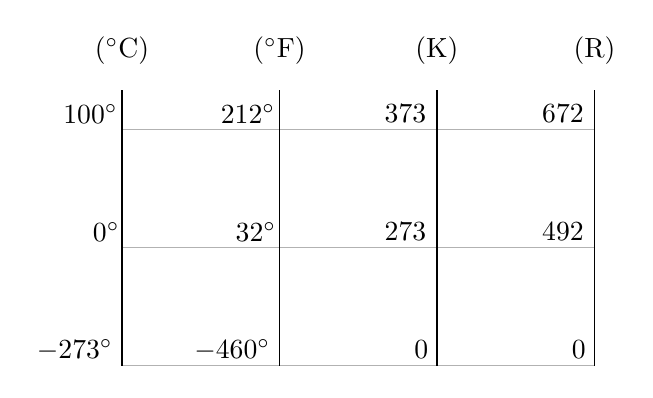
\begin{tikzpicture}
		\draw[draw=black!30] (0,0) -- (6,0);
		\draw[draw=black!30] (0,1.5) -- (6,1.5);
		\draw[draw=black!30] (0,3) -- (6,3);
		\draw (0,0) -- (0,3.5);
		\draw (2,0) -- (2,3.5);
		\draw (4,0) -- (4,3.5);
		\draw (6,0) -- (6,3.5);
		\node at (0,4) {$\mathrm{(^\circ C)}$};
		\node at (2,4) {$\mathrm{(^\circ F)}$};
		\node at (4,4) {$\mathrm{(K)}$};
		\node at (6,4) {$\mathrm{(R)}$};
		\node at (-0.6,0.2) {$-273^\circ$};
		\node at (-0.2,1.7) {$0^\circ$};
		\node at (-0.4,3.2) {$100^\circ$};
		\node at (1.4,0.2) {$-460^\circ$};
		\node at (1.7,1.7) {$32^\circ$};
		\node at (1.6,3.2) {$212^\circ$};
		\node at (3.8,0.2) {$0$};
		\node at (3.6,1.7) {$273$};
		\node at (3.6,3.2) {$373$};
		\node at (5.8,0.2) {$0$};
		\node at (5.6,1.7) {$492$};
		\node at (5.6,3.2) {$672$};
	\end{tikzpicture}
\end{figure}
entonces su forma de relacion se da de la siguiente manera:
$$ \frac{^\circ C}{5}=\frac{^\circ F-32}{9}=\frac{K-273}{5}=\frac{R-492}{9} $$
y su relacion de variacion se da de la siguiente manera:
$$ \frac{\Delta C}{5}=\frac{\Delta F}{9}=\frac{\Delta K}{5}=\frac{\Delta R}{9} $$